\chapter{Conceitos básicos sobre grafos}

Muitos problemas de programação podem ser resolvidos modelando o problema como um problema de grafo e usando um algoritmo de grafo apropriado. Um exemplo típico de grafo é uma rede de estradas e cidades em um país. Às vezes, porém, o grafo está oculto no problema e pode ser difícil detectá-lo.

Esta parte do livro discute algoritmos de grafos, com foco especial em tópicos que são importantes na programação competitiva. Neste capítulo, abordaremos conceitos relacionados a grafos e estudaremos diferentes maneiras de representar grafos em algoritmos.

\section{Terminologia de grafos}

\index{grafo}
\index{nó}
\index{aresta}

Um \key{grafo} consiste em \key{nós} e \key{arestas}. Neste livro, a variável $n$ denota o número de nós em um grafo, e a variável $m$ denota o número de arestas. Os nós são numerados usando inteiros $1,2,\ldots,n$.

Por exemplo, o grafo a seguir consiste em 5 nós e 7 arestas:

\begin{center}
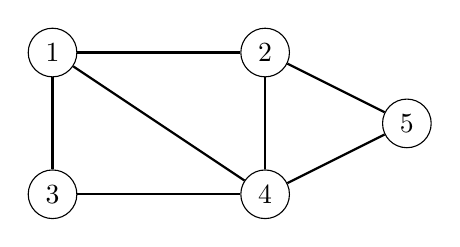
\begin{tikzpicture}[scale=0.9]
\node[draw, circle] (1) at (1,3) {$1$};
\node[draw, circle] (2) at (4,3) {$2$};
\node[draw, circle] (3) at (1,1) {$3$};
\node[draw, circle] (4) at (4,1) {$4$};
\node[draw, circle] (5) at (6,2) {$5$};

\path[draw,thick,-] (1) -- (2);
\path[draw,thick,-] (1) -- (3);
\path[draw,thick,-] (1) -- (4);
\path[draw,thick,-] (3) -- (4);
\path[draw,thick,-] (2) -- (4);
\path[draw,thick,-] (2) -- (5);
\path[draw,thick,-] (4) -- (5);
\end{tikzpicture}
\end{center}

\index{caminho}

Um \key{caminho} leva do nó $a$ ao nó $b$ através das arestas do grafo. O \key{comprimento} de um caminho é o número de arestas nele. Por exemplo, o grafo acima contém um caminho $1 \rightarrow 3 \rightarrow 4 \rightarrow 5$ de comprimento 3 do nó 1 ao nó 5:

\begin{center}
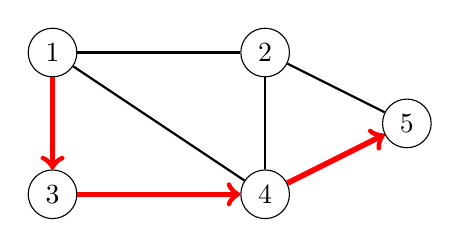
\begin{tikzpicture}[scale=0.9]
\node[draw, circle] (1) at (1,3) {$1$};
\node[draw, circle] (2) at (4,3) {$2$};
\node[draw, circle] (3) at (1,1) {$3$};
\node[draw, circle] (4) at (4,1) {$4$};
\node[draw, circle] (5) at (6,2) {$5$};

\path[draw,thick,-] (1) -- (2);
\path[draw,thick,-] (1) -- (3);
\path[draw,thick,-] (1) -- (4);
\path[draw,thick,-] (3) -- (4);
\path[draw,thick,-] (2) -- (4);
\path[draw,thick,-] (2) -- (5);
\path[draw,thick,-] (4) -- (5);

\path[draw=red,thick,->,line width=2pt] (1) -- (3);
\path[draw=red,thick,->,line width=2pt] (3) -- (4);
\path[draw=red,thick,->,line width=2pt] (4) -- (5);
\end{tikzpicture}
\end{center}

\index{ciclo}

Um caminho é um \key{ciclo} se o primeiro e o último nó forem os mesmos. Por exemplo, o grafo acima contém um ciclo $1 \rightarrow 3 \rightarrow 4 \rightarrow 1$. Um caminho é \key{simples} se cada nó aparecer no máximo uma vez no caminho.


% 
% \begin{itemize}
% \item $1 \rightarrow 2 \rightarrow 5$ (length 2)
% \item $1 \rightarrow 4 \rightarrow 5$ (length 2)
% \item $1 \rightarrow 2 \rightarrow 4 \rightarrow 5$ (length 3)
% \item $1 \rightarrow 3 \rightarrow 4 \rightarrow 5$ (length 3)
% \item $1 \rightarrow 4 \rightarrow 2 \rightarrow 5$ (length 3)
% \item $1 \rightarrow 3 \rightarrow 4 \rightarrow 2 \rightarrow 5$ (length 4)
% \end{itemize}

\subsubsection{Conectividade}

\index{grafo conexo}

Um grafo é \key{conexo} se houver um caminho entre quaisquer dois nós. Por exemplo, o seguinte grafo é conexo:
\begin{center}
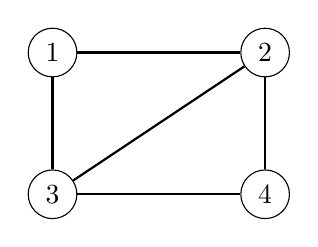
\begin{tikzpicture}[scale=0.9]
\node[draw, circle] (1) at (1,3) {$1$};
\node[draw, circle] (2) at (4,3) {$2$};
\node[draw, circle] (3) at (1,1) {$3$};
\node[draw, circle] (4) at (4,1) {$4$};
\path[draw,thick,-] (1) -- (2);
\path[draw,thick,-] (1) -- (3);
\path[draw,thick,-] (2) -- (3);
\path[draw,thick,-] (3) -- (4);
\path[draw,thick,-] (2) -- (4);
\end{tikzpicture}
\end{center}

O seguinte grafo não é conexo, porque não é possível ir do nó 4 a nenhum outro nó:
\begin{center}
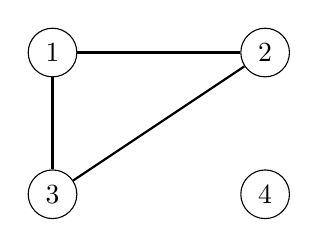
\begin{tikzpicture}[scale=0.9]
\node[draw, circle] (1) at (1,3) {$1$};
\node[draw, circle] (2) at (4,3) {$2$};
\node[draw, circle] (3) at (1,1) {$3$};
\node[draw, circle] (4) at (4,1) {$4$};
\path[draw,thick,-] (1) -- (2);
\path[draw,thick,-] (1) -- (3);
\path[draw,thick,-] (2) -- (3);
\end{tikzpicture}
\end{center}

\index{componente}

As partes conectadas de um grafo são chamadas de seus \key{componentes}. Por exemplo, o seguinte grafo contém três componentes:
$\{1,\,2,\,3\}$,
$\{4,\,5,\,6,\,7\}$ e
$\{8\}$.
\begin{center}
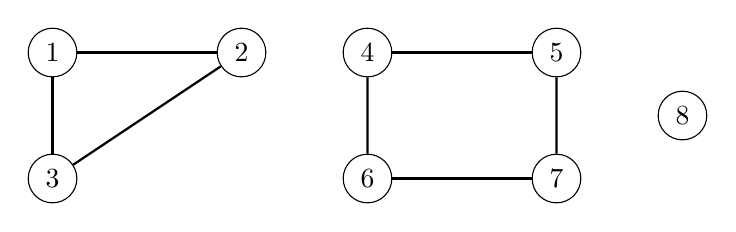
\begin{tikzpicture}[scale=0.8]
\node[draw, circle] (1) at (1,3) {$1$};
\node[draw, circle] (2) at (4,3) {$2$};
\node[draw, circle] (3) at (1,1) {$3$};

\node[draw, circle] (6) at (6,1) {$6$};
\node[draw, circle] (7) at (9,1) {$7$};
\node[draw, circle] (4) at (6,3) {$4$};
\node[draw, circle] (5) at (9,3) {$5$};

\node[draw, circle] (8) at (11,2) {$8$};

\path[draw,thick,-] (1) -- (2);
\path[draw,thick,-] (2) -- (3);
\path[draw,thick,-] (1) -- (3);
\path[draw,thick,-] (4) -- (5);
\path[draw,thick,-] (5) -- (7);
\path[draw,thick,-] (6) -- (7);
\path[draw,thick,-] (6) -- (4);
\end{tikzpicture}
\end{center}

\index{árvore}

Uma \key{árvore} é um grafo conexo que consiste em $n$ nós e $n-1$ arestas. Existe um único caminho entre quaisquer dois nós de uma árvore. Por exemplo, o seguinte grafo é uma árvore:

\begin{center}
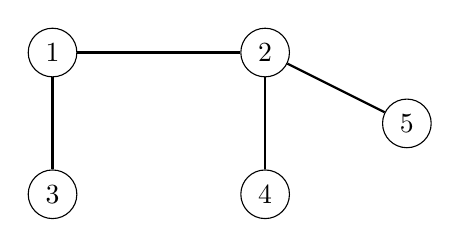
\begin{tikzpicture}[scale=0.9]
\node[draw, circle] (1) at (1,3) {$1$};
\node[draw, circle] (2) at (4,3) {$2$};
\node[draw, circle] (3) at (1,1) {$3$};
\node[draw, circle] (4) at (4,1) {$4$};
\node[draw, circle] (5) at (6,2) {$5$};

\path[draw,thick,-] (1) -- (2);
\path[draw,thick,-] (1) -- (3);
%\path[draw,thick,-] (1) -- (4);
\path[draw,thick,-] (2) -- (5);
\path[draw,thick,-] (2) -- (4);
%\path[draw,thick,-] (4) -- (5);
\end{tikzpicture}
\end{center}

\subsubsection{Direções das arestas}

\index{grafo direcionado}

Um grafo é \key{direcionado} se as arestas puderem ser percorridas em apenas uma direção. Por exemplo, o seguinte grafo é direcionado:
\begin{center}
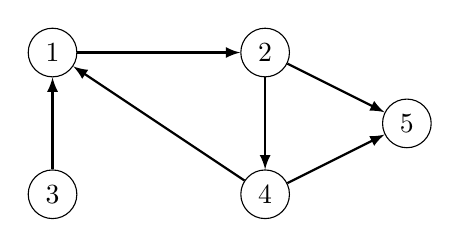
\begin{tikzpicture}[scale=0.9]
\node[draw, circle] (1) at (1,3) {$1$};
\node[draw, circle] (2) at (4,3) {$2$};
\node[draw, circle] (3) at (1,1) {$3$};
\node[draw, circle] (4) at (4,1) {$4$};
\node[draw, circle] (5) at (6,2) {$5$};
\path[draw,thick,->,>=latex] (1) -- (2);
\path[draw,thick,->,>=latex] (2) -- (4);
\path[draw,thick,->,>=latex] (2) -- (5);
\path[draw,thick,->,>=latex] (4) -- (5);
\path[draw,thick,->,>=latex] (4) -- (1);
\path[draw,thick,->,>=latex] (3) -- (1);
\end{tikzpicture}
\end{center}

O grafo acima contém um caminho $3 \rightarrow 1 \rightarrow 2 \rightarrow 5$ do nó $3$ ao nó $5$, mas não há caminho do nó $5$ ao nó $3$.

\subsubsection{Pesos das arestas}

\index{grafo ponderado}

Em um grafo \key{ponderado}, cada aresta recebe um \key{peso}. Os pesos são frequentemente interpretados como comprimentos de aresta. Por exemplo, o seguinte grafo é ponderado:
\begin{center}
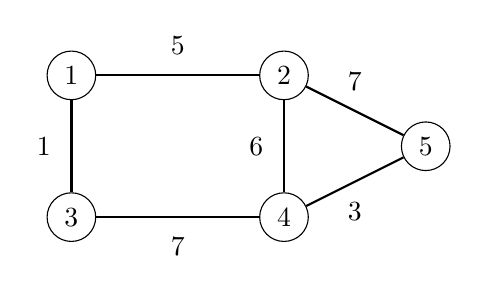
\begin{tikzpicture}[scale=0.9]
\node[draw, circle] (1) at (1,3) {$1$};
\node[draw, circle] (2) at (4,3) {$2$};
\node[draw, circle] (3) at (1,1) {$3$};
\node[draw, circle] (4) at (4,1) {$4$};
\node[draw, circle] (5) at (6,2) {$5$};
\path[draw,thick,-] (1) -- node[font=\small,label=above:5] {} (2);
\path[draw,thick,-] (1) -- node[font=\small,label=left:1] {} (3);
\path[draw,thick,-] (3) -- node[font=\small,label=below:7] {} (4);
\path[draw,thick,-] (2) -- node[font=\small,label=left:6] {} (4);
\path[draw,thick,-] (2) -- node[font=\small,label=above:7] {} (5);
\path[draw,thick,-] (4) -- node[font=\small,label=below:3] {} (5);
\end{tikzpicture}
\end{center}

O comprimento de um caminho em um grafo ponderado é a soma dos pesos das arestas no caminho. Por exemplo, no grafo acima, o comprimento do caminho
$1 \rightarrow 2 \rightarrow 5$ é $12$,
e o comprimento do caminho
$1 \rightarrow 3 \rightarrow 4 \rightarrow 5$ é $11$.
O último caminho é o \key{caminho mais curto} do nó $1$ ao nó $5$.

\subsubsection{Vizinhos e graus}

\index{vizinho}
\index{grau}

Dois nós são \key{vizinhos} ou \key{adjacentes} se houver uma aresta entre eles. O \key{grau} de um nó é o número de seus vizinhos. Por exemplo, no seguinte grafo, os vizinhos do nó 2 são 1, 4 e 5, então seu grau é 3.

\begin{center}
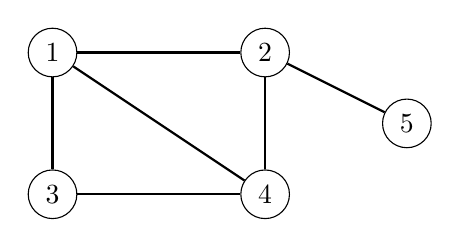
\begin{tikzpicture}[scale=0.9]
\node[draw, circle] (1) at (1,3) {$1$};
\node[draw, circle] (2) at (4,3) {$2$};
\node[draw, circle] (3) at (1,1) {$3$};
\node[draw, circle] (4) at (4,1) {$4$};
\node[draw, circle] (5) at (6,2) {$5$};

\path[draw,thick,-] (1) -- (2);
\path[draw,thick,-] (1) -- (3);
\path[draw,thick,-] (1) -- (4);
\path[draw,thick,-] (3) -- (4);
\path[draw,thick,-] (2) -- (4);
\path[draw,thick,-] (2) -- (5);
%\path[draw,thick,-] (4) -- (5);
\end{tikzpicture}
\end{center}

A soma dos graus em um grafo é sempre $2m$, onde $m$ é o número de arestas, porque cada aresta aumenta em um o grau de exatamente dois nós. Por esta razão, a soma dos graus é sempre par.

\index{grafo regular}
\index{grafo completo}

Um grafo é \key{regular} se o grau de cada nó for uma constante $d$. Um grafo é \key{completo} se o grau de cada nó for $n-1$, ou seja, o grafo contém todas as arestas possíveis entre os nós.

\index{grau de entrada}
\index{grau de saída}

Em um grafo direcionado, o \key{grau de entrada} de um nó é o número de arestas que terminam no nó, e o \key{grau de saída} de um nó é o número de arestas que começam no nó. Por exemplo, no seguinte grafo, o grau de entrada do nó 2 é 2, e o grau de saída do nó 2 é 1.

\begin{center}
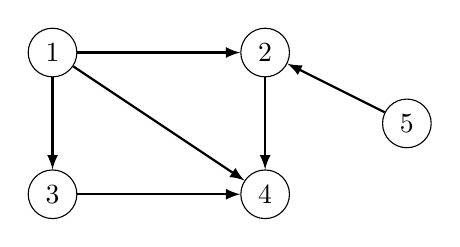
\begin{tikzpicture}[scale=0.9]
\node[draw, circle] (1) at (1,3) {$1$};
\node[draw, circle] (2) at (4,3) {$2$};
\node[draw, circle] (3) at (1,1) {$3$};
\node[draw, circle] (4) at (4,1) {$4$};
\node[draw, circle] (5) at (6,2) {$5$};

\path[draw,thick,->,>=latex] (1) -- (2);
\path[draw,thick,->,>=latex] (1) -- (3);
\path[draw,thick,->,>=latex] (1) -- (4);
\path[draw,thick,->,>=latex] (3) -- (4);
\path[draw,thick,->,>=latex] (2) -- (4);
\path[draw,thick,<-,>=latex] (2) -- (5);
\end{tikzpicture}
\end{center}

\subsubsection{Colorações}

\index{coloração}
\index{grafo bipartido}

Em uma \key{coloração} de um grafo, cada nó recebe uma cor de forma que nenhum nó adjacente tenha a mesma cor.

Um grafo é \key{bipartido} se for possível colori-lo usando duas cores. Acontece que um grafo é bipartido exatamente quando não contém um ciclo com um número ímpar de arestas. Por exemplo, o grafo
\begin{center}
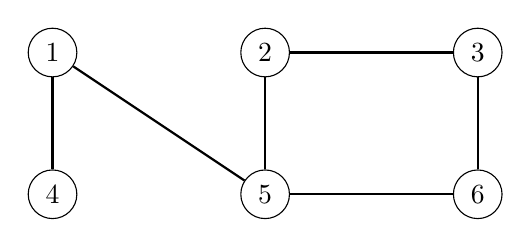
\begin{tikzpicture}[scale=0.9]
\node[draw, circle] (1) at (1,3) {$2$};
\node[draw, circle] (2) at (4,3) {$3$};
\node[draw, circle] (3) at (1,1) {$5$};
\node[draw, circle] (4) at (4,1) {$6$};
\node[draw, circle] (5) at (-2,1) {$4$};
\node[draw, circle] (6) at (-2,3) {$1$};
\path[draw,thick,-] (1) -- (2);
\path[draw,thick,-] (1) -- (3);
\path[draw,thick,-] (3) -- (4);
\path[draw,thick,-] (2) -- (4);
\path[draw,thick,-] (3) -- (6);
\path[draw,thick,-] (5) -- (6);
\end{tikzpicture}
\end{center}
é bipartido, pois pode ser colorido da seguinte forma:
\begin{center}
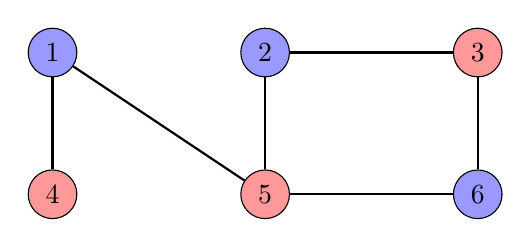
\begin{tikzpicture}[scale=0.9]
\node[draw, circle, fill=blue!40] (1) at (1,3) {$2$};
\node[draw, circle, fill=red!40] (2) at (4,3) {$3$};
\node[draw, circle, fill=red!40] (3) at (1,1) {$5$};
\node[draw, circle, fill=blue!40] (4) at (4,1) {$6$};
\node[draw, circle, fill=red!40] (5) at (-2,1) {$4$};
\node[draw, circle, fill=blue!40] (6) at (-2,3) {$1$};
\path[draw,thick,-] (1) -- (2);
\path[draw,thick,-] (1) -- (3);
\path[draw,thick,-] (3) -- (4);
\path[draw,thick,-] (2) -- (4);
\path[draw,thick,-] (3) -- (6);
\path[draw,thick,-] (5) -- (6);
\end{tikzpicture}
\end{center}
No entanto, o grafo
\begin{center}
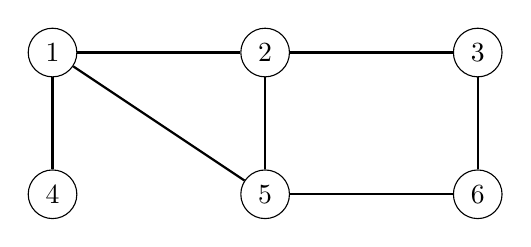
\begin{tikzpicture}[scale=0.9]
\node[draw, circle] (1) at (1,3) {$2$};
\node[draw, circle] (2) at (4,3) {$3$};
\node[draw, circle] (3) at (1,1) {$5$};
\node[draw, circle] (4) at (4,1) {$6$};
\node[draw, circle] (5) at (-2,1) {$4$};
\node[draw, circle] (6) at (-2,3) {$1$};
\path[draw,thick,-] (1) -- (2);
\path[draw,thick,-] (1) -- (3);
\path[draw,thick,-] (3) -- (4);
\path[draw,thick,-] (2) -- (4);
\path[draw,thick,-] (3) -- (6);
\path[draw,thick,-] (5) -- (6);
\path[draw,thick,-] (1) -- (6);
\end{tikzpicture}
\end{center}
não é bipartido, porque não é possível colorir o seguinte ciclo de três nós usando duas cores:
\begin{center}
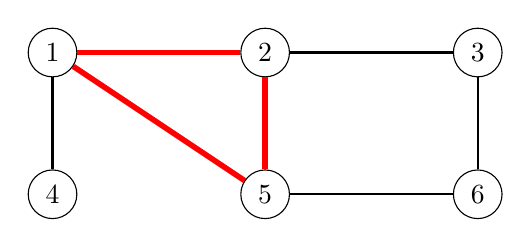
\begin{tikzpicture}[scale=0.9]
\node[draw, circle] (1) at (1,3) {$2$};
\node[draw, circle] (2) at (4,3) {$3$};
\node[draw, circle] (3) at (1,1) {$5$};
\node[draw, circle] (4) at (4,1) {$6$};
\node[draw, circle] (5) at (-2,1) {$4$};
\node[draw, circle] (6) at (-2,3) {$1$};
\path[draw,thick,-] (1) -- (2);
\path[draw,thick,-] (1) -- (3);
\path[draw,thick,-] (3) -- (4);
\path[draw,thick,-] (2) -- (4);
\path[draw,thick,-] (3) -- (6);
\path[draw,thick,-] (5) -- (6);
\path[draw,thick,-] (1) -- (6);

\path[draw=red,thick,-,line width=2pt] (1) -- (3);
\path[draw=red,thick,-,line width=2pt] (3) -- (6);
\path[draw,red,thick,-,line width=2pt] (6) -- (1);
\end{tikzpicture}
\end{center}

\subsubsection{Simplicidade}

\index{grafo simples}

Um grafo é \key{simples} se nenhuma aresta começa e termina no mesmo nó, e não há múltiplas arestas entre dois nós. Muitas vezes, assumimos que os grafos são simples. Por exemplo, o seguinte grafo \emph{não} é simples:
\begin{center}
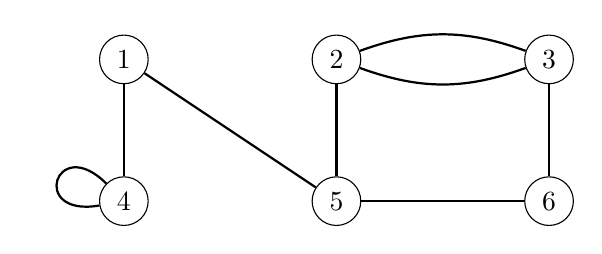
\begin{tikzpicture}[scale=0.9]
\node[draw, circle] (1) at (1,3) {$2$};
\node[draw, circle] (2) at (4,3) {$3$};
\node[draw, circle] (3) at (1,1) {$5$};
\node[draw, circle] (4) at (4,1) {$6$};
\node[draw, circle] (5) at (-2,1) {$4$};
\node[draw, circle] (6) at (-2,3) {$1$};

\path[draw,thick,-] (1) edge [bend right=20] (2);
\path[draw,thick,-] (2) edge [bend right=20] (1);
%\path[draw,thick,-] (1) -- (2);
\path[draw,thick,-] (1) -- (3);
\path[draw,thick,-] (3) -- (4);
\path[draw,thick,-] (2) -- (4);
\path[draw,thick,-] (3) -- (6);
\path[draw,thick,-] (5) -- (6);

\tikzset{every loop/.style={in=135,out=190}}
\path[draw,thick,-] (5) edge [loop left] (5);
\end{tikzpicture}
\end{center}

\section{Representação de grafos}

Existem várias maneiras de representar grafos em algoritmos. A escolha de uma estrutura de dados depende do tamanho do grafo e da maneira como o algoritmo o processa. A seguir, veremos três representações comuns.

\subsubsection{Representação de lista de adjacência}

\index{lista de adjacência}

Na representação de lista de adjacência, cada nó $x$ no grafo recebe uma \key{lista de adjacência} que consiste em nós para os quais há uma aresta de $x$. Listas de adjacência são a maneira mais popular de representar grafos, e a maioria dos algoritmos pode ser implementada de forma eficiente usando-as.

Uma maneira conveniente de armazenar as listas de adjacência é declarar um array de vetores da seguinte forma:
\begin{lstlisting}
vector<int> adj[N];
\end{lstlisting}

A constante $N$ é escolhida de forma que todas as listas de adjacência possam ser armazenadas. Por exemplo, o grafo

\begin{center}
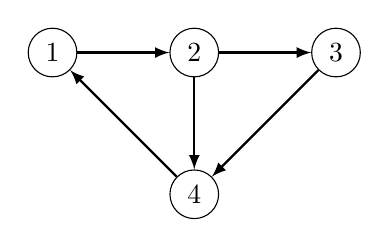
\begin{tikzpicture}[scale=0.9]
\node[draw, circle] (1) at (1,3) {$1$};
\node[draw, circle] (2) at (3,3) {$2$};
\node[draw, circle] (3) at (5,3) {$3$};
\node[draw, circle] (4) at (3,1) {$4$};

\path[draw,thick,->,>=latex] (1) -- (2);
\path[draw,thick,->,>=latex] (2) -- (3);
\path[draw,thick,->,>=latex] (2) -- (4);
\path[draw,thick,->,>=latex] (3) -- (4);
\path[draw,thick,->,>=latex] (4) -- (1);
\end{tikzpicture}
\end{center}
pode ser armazenado da seguinte forma:
\begin{lstlisting}
adj[1].push_back(2);
adj[2].push_back(3);
adj[2].push_back(4);
adj[3].push_back(4);
adj[4].push_back(1);
\end{lstlisting}

Se o grafo for não direcionado, ele pode ser armazenado de forma semelhante, mas cada aresta é adicionada em ambas as direções.

Para um grafo ponderado, a estrutura pode ser estendida da seguinte forma:

\begin{lstlisting}
vector<pair<int,int>> adj[N];
\end{lstlisting}

Nesse caso, a lista de adjacência do nó $a$ contém o par $(b,w)$ sempre que houver uma aresta do nó $a$ ao nó $b$ com peso $w$. Por exemplo, o grafo

\begin{center}
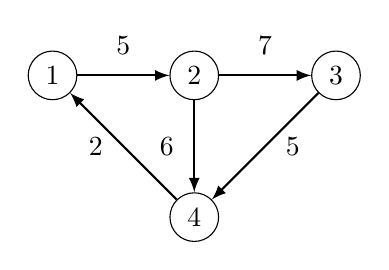
\begin{tikzpicture}[scale=0.9]
\node[draw, circle] (1) at (1,3) {$1$};
\node[draw, circle] (2) at (3,3) {$2$};
\node[draw, circle] (3) at (5,3) {$3$};
\node[draw, circle] (4) at (3,1) {$4$};

\path[draw,thick,->,>=latex] (1) -- node[font=\small,label=above:5] {} (2);
\path[draw,thick,->,>=latex] (2) -- node[font=\small,label=above:7] {} (3);
\path[draw,thick,->,>=latex] (2) -- node[font=\small,label=left:6] {} (4);
\path[draw,thick,->,>=latex] (3) -- node[font=\small,label=right:5] {} (4);
\path[draw,thick,->,>=latex] (4) -- node[font=\small,label=left:2] {} (1);
\end{tikzpicture}
\end{center}
pode ser armazenado da seguinte forma:
\begin{lstlisting}
adj[1].push_back({2,5});
adj[2].push_back({3,7});
adj[2].push_back({4,6});
adj[3].push_back({4,5});
adj[4].push_back({1,2});
\end{lstlisting}

O benefício de usar listas de adjacência é que podemos encontrar os nós para os quais podemos mover de um determinado nó através de uma aresta de forma eficiente. Por exemplo, o seguinte loop percorre todos os nós para os quais podemos mover do nó $s$:

\begin{lstlisting}
for (auto u : adj[s]) {
    // processa o no u
}
\end{lstlisting}

\subsubsection{Representação de matriz de adjacência}

\index{matriz de adjacência}

Uma \key{matriz de adjacência} é um array bidimensional que indica quais arestas o grafo contém. Podemos verificar eficientemente a partir de uma matriz de adjacência se existe uma aresta entre dois nós. A matriz pode ser armazenada como um array
\begin{lstlisting}
int adj[N][N];
\end{lstlisting}
onde cada valor $\texttt{adj}[a][b]$ indica se o grafo contém uma aresta do nó $a$ ao nó $b$. Se a aresta estiver incluída no grafo, então $\texttt{adj}[a][b]=1$, e caso contrário $\texttt{adj}[a][b]=0$. Por exemplo, o grafo
\begin{center}
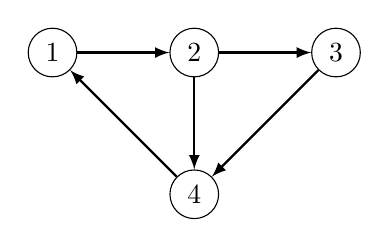
\begin{tikzpicture}[scale=0.9]
\node[draw, circle] (1) at (1,3) {$1$};
\node[draw, circle] (2) at (3,3) {$2$};
\node[draw, circle] (3) at (5,3) {$3$};
\node[draw, circle] (4) at (3,1) {$4$};

\path[draw,thick,->,>=latex] (1) -- (2);
\path[draw,thick,->,>=latex] (2) -- (3);
\path[draw,thick,->,>=latex] (2) -- (4);
\path[draw,thick,->,>=latex] (3) -- (4);
\path[draw,thick,->,>=latex] (4) -- (1);
\end{tikzpicture}
\end{center}
pode ser representado da seguinte forma:
\begin{center}
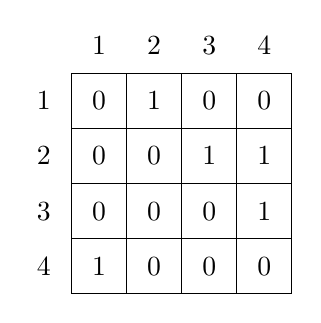
\begin{tikzpicture}[scale=0.7]
\draw (0,0) grid (4,4);
\node at (0.5,0.5) {1};
\node at (1.5,0.5) {0};
\node at (2.5,0.5) {0};
\node at (3.5,0.5) {0};
\node at (0.5,1.5) {0};
\node at (1.5,1.5) {0};
\node at (2.5,1.5) {0};
\node at (3.5,1.5) {1};
\node at (0.5,2.5) {0};
\node at (1.5,2.5) {0};
\node at (2.5,2.5) {1};
\node at (3.5,2.5) {1};
\node at (0.5,3.5) {0};
\node at (1.5,3.5) {1};
\node at (2.5,3.5) {0};
\node at (3.5,3.5) {0};
\node at (-0.5,0.5) {4};
\node at (-0.5,1.5) {3};
\node at (-0.5,2.5) {2};
\node at (-0.5,3.5) {1};
\node at (0.5,4.5) {1};
\node at (1.5,4.5) {2};
\node at (2.5,4.5) {3};
\node at (3.5,4.5) {4};
\end{tikzpicture}
\end{center}

Se o grafo for ponderado, a representação da matriz de adjacência pode ser estendida para que a matriz contenha o peso da aresta, se a aresta existir. Usando essa representação, o grafo

\begin{center}
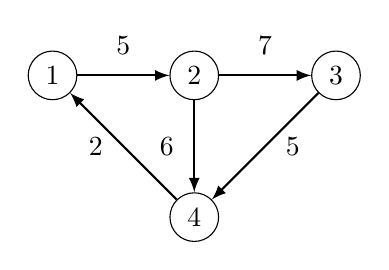
\begin{tikzpicture}[scale=0.9]
\node[draw, circle] (1) at (1,3) {$1$};
\node[draw, circle] (2) at (3,3) {$2$};
\node[draw, circle] (3) at (5,3) {$3$};
\node[draw, circle] (4) at (3,1) {$4$};

\path[draw,thick,->,>=latex] (1) -- node[font=\small,label=above:5] {} (2);
\path[draw,thick,->,>=latex] (2) -- node[font=\small,label=above:7] {} (3);
\path[draw,thick,->,>=latex] (2) -- node[font=\small,label=left:6] {} (4);
\path[draw,thick,->,>=latex] (3) -- node[font=\small,label=right:5] {} (4);
\path[draw,thick,->,>=latex] (4) -- node[font=\small,label=left:2] {} (1);
\end{tikzpicture}
\end{center}
\begin{samepage}
corresponde à seguinte matriz:
\begin{center}
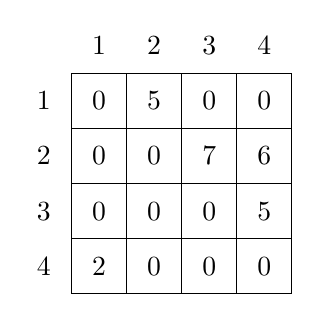
\begin{tikzpicture}[scale=0.7]
\draw (0,0) grid (4,4);
\node at (0.5,0.5) {2};
\node at (1.5,0.5) {0};
\node at (2.5,0.5) {0};
\node at (3.5,0.5) {0};
\node at (0.5,1.5) {0};
\node at (1.5,1.5) {0};
\node at (2.5,1.5) {0};
\node at (3.5,1.5) {5};
\node at (0.5,2.5) {0};
\node at (1.5,2.5) {0};
\node at (2.5,2.5) {7};
\node at (3.5,2.5) {6};
\node at (0.5,3.5) {0};
\node at (1.5,3.5) {5};
\node at (2.5,3.5) {0};
\node at (3.5,3.5) {0};
\node at (-0.5,0.5) {4};
\node at (-0.5,1.5) {3};
\node at (-0.5,2.5) {2};
\node at (-0.5,3.5) {1};
\node at (0.5,4.5) {1};
\node at (1.5,4.5) {2};
\node at (2.5,4.5) {3};
\node at (3.5,4.5) {4};
\end{tikzpicture}
\end{center}
\end{samepage}

A desvantagem da representação da matriz de adjacência é que a matriz contém $n^2$ elementos e, geralmente, a maioria deles é zero. Por esse motivo, a representação não pode ser usada se o gráfico for grande.

\subsubsection{Representação de lista de arestas}

\index{lista de arestas}

Uma \key{lista de arestas} contém todas as arestas de um grafo em alguma ordem. Esta é uma maneira conveniente de representar um grafo se o algoritmo processa todas as arestas do grafo e não é necessário encontrar arestas que comecem em um determinado nó.

A lista de arestas pode ser armazenada em um vetor
\begin{lstlisting}
vector<pair<int,int>> edges;
\end{lstlisting}
onde cada par $(a,b)$ denota que há uma aresta do nó $a$ ao nó $b$. Assim, o grafo

\begin{center}
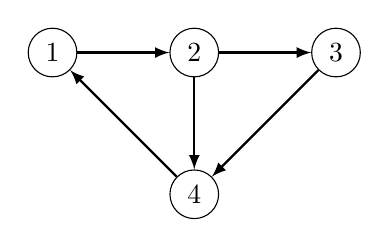
\begin{tikzpicture}[scale=0.9]
\node[draw, circle] (1) at (1,3) {$1$};
\node[draw, circle] (2) at (3,3) {$2$};
\node[draw, circle] (3) at (5,3) {$3$};
\node[draw, circle] (4) at (3,1) {$4$};

\path[draw,thick,->,>=latex] (1) -- (2);
\path[draw,thick,->,>=latex] (2) -- (3);
\path[draw,thick,->,>=latex] (2) -- (4);
\path[draw,thick,->,>=latex] (3) -- (4);
\path[draw,thick,->,>=latex] (4) -- (1);
\end{tikzpicture}
\end{center}
pode ser representado da seguinte forma:
\begin{lstlisting}
edges.push_back({1,2});
edges.push_back({2,3});
edges.push_back({2,4});
edges.push_back({3,4});
edges.push_back({4,1});
\end{lstlisting}

\noindent
Se o grafo for ponderado, a estrutura pode ser estendida da seguinte forma:
\begin{lstlisting}
vector<tuple<int,int,int>> edges;
\end{lstlisting}
Cada elemento desta lista é da forma $(a,b,w)$, o que significa que há uma aresta do nó $a$ ao nó $b$ com peso $w$. Por exemplo, o grafo

\begin{center}
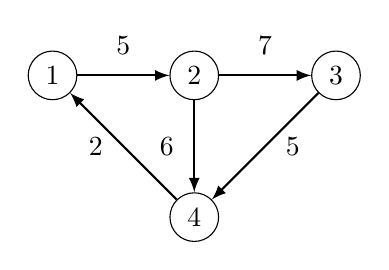
\begin{tikzpicture}[scale=0.9]
\node[draw, circle] (1) at (1,3) {$1$};
\node[draw, circle] (2) at (3,3) {$2$};
\node[draw, circle] (3) at (5,3) {$3$};
\node[draw, circle] (4) at (3,1) {$4$};

\path[draw,thick,->,>=latex] (1) -- node[font=\small,label=above:5] {} (2);
\path[draw,thick,->,>=latex] (2) -- node[font=\small,label=above:7] {} (3);
\path[draw,thick,->,>=latex] (2) -- node[font=\small,label=left:6] {} (4);
\path[draw,thick,->,>=latex] (3) -- node[font=\small,label=right:5] {} (4);
\path[draw,thick,->,>=latex] (4) -- node[font=\small,label=left:2] {} (1);
\end{tikzpicture}
\end{center}
\begin{samepage}
pode ser representado da seguinte forma\footnote{Em alguns compiladores mais antigos, a função
\texttt{make\_tuple} deve ser usada no lugar das chaves (por exemplo,
\texttt{make\_tuple(1,2,5)} em vez de \texttt{\{1,2,5\}}).}:
\begin{lstlisting}
edges.push_back({1,2,5});
edges.push_back({2,3,7});
edges.push_back({2,4,6});
edges.push_back({3,4,5});
edges.push_back({4,1,2});
\end{lstlisting}
\end{samepage}
